\documentclass[../dissertation.tex]{subfiles}
\begin{document}
Now that gradient flow equation and tangent-point energy are introduced,
one can formalise the process of untangling a tangled curve:

\begin{definition}[Curve Untangling Process]
    Given a parameterised curve $\gammabf:M \times T \rightarrow \mathbb{R}^3$ over an interval $M$ and time domain $T$,
    denote the following initial value problem as \textbf{curve untangling process}:
    \begin{align}
        \frac{\partial \gammabf}{\partial t} &= - \grad_{\mathcal{X}} \mathcal{E}_{\beta}^{\alpha} (\gammabf) - \grad_{\mathcal{X}} \mathcal{C} (\gammabf) 
        \label{equ: Curve Untangling Process}
        \\
        \gammabf(s;0) &= \gammabf_0 (s)
        \label{equ: Initial Curve}
    \end{align}
    where 
    \begin{itemize}
        \item $\gammabf_0 (s)$ is the parameterisation of the initial (tangled) curve (prescribed at $t=0$)
        \item $\mathcal{E}_{\beta}^{\alpha}$ is the tangent-point energy (See (\ref{equ: Tangent-Point Energy}))
        \item $\mathcal{C}$ is additional constraint energy to control behaviour of curve untangling process.
    \end{itemize}
\end{definition}

\section{Constraint Energy}
From lemma \ref{lemma: Scale-Invariance}, in the case that $\beta > \alpha + 2$,
one could trivially minimise tangent-point energy $\mathcal{E}_{\beta}^{\alpha}$ of the curve by scaling the curve to infinity.
In order to avoid this phenomenon, or to change the behaviour of the flow, one may add additional energy which penalises unwanted behaviours.
\begin{itemize}
    \item Taking $\mathcal{C} \coloneqq \lambda \int_{M} \norm{\gammabf}^{p} \intd \gamma$ adds the motivation for the curve not to stray away from the origin.
        \begin{itemize}
            \item $\lambda > 0$ is the strength of the overall constraint.
            \item $p > 0$ is the order of local strength, where higher $p$ would lead to harsher ``thresholding''.
        \end{itemize}
\end{itemize}


\subsection{Discretisation for Numerical Computation}
Solving (\ref{equ: Curve Untangling Process}), (\ref{equ: Initial Curve}) analytically is challenging.
Rather, we aim to acquire a numerical solution.
Assume for simplicity that the curve of interest is simple closed.\footnote{
    We may assume that the function definition of $\gammabf:M \rightarrow \mathbb{R}^3$ extends to $\gammabf: \mathbb{R} \rightarrow \mathbb{R}^3$ by periodicity.
}

\subsubsection{Discretisation of Curve}
We start by discretising the initial curve $\gammabf_0$ by taking $N$ points on a curve as shown in Figure \ref{fig: Discretization of Curve}.
Represent the initially discretised curve as $\Gammabf^0 = \left( \xbf_0^0, \xbf_1^0, \cdots, \xbf_{N-1}^0 \right)$,
and the discretised curve at time step $k \in \mathbb{N} \cup \left\{ 0 \right\}$ as $\Gammabf^k = \left( \xbf_0^k, \xbf_1^k, \cdots, \xbf_{N-1}^k \right)$.
Since we restrict our attention to a simple closed curve, it is convenient to extend the indexing rule by:
\begin{equation}
    \xbf_{i}^k = \xbf_{r\left( i,N \right)}^k \hspace{1cm} \text{where } r\left( i,N \right) = \text{(remainder of } i \div N \text{)}
\end{equation}
so that $\xbf_N^k = \xbf_{0}^k$, $\xbf_{N+1}^k = \xbf_{1}^k$, etc.

Assign a function definition $\Gammabf^k: \mathbb{Z} \rightarrow \left\{ \xbf_0^k, \xbf_1^k, \cdots, \xbf_{N-1}^k \right\}$ as:
\begin{equation}
    \Gammabf^k (i) = \xbf_{r\left( i, N \right)}^k 
\end{equation}
anaogous to $\gammabf = \gammabf(s)$ being a parameterised curve, which is a vector-valued function.

Finally, denote by $e_{i}^k$ for the (undirected) edge with vertex pair $\left( \xbf_i^k, \xbf_{i+1}^k \right)$.

\subsubsection{Discretisation of Tangent-Point Energy}
In order to acquire numerical solution, one must also be able to numerically compute the tangent-point energy.
For this, we pose the energy quadrature $E_{\beta}^{\alpha} \left( \Gammabf \right)$ of the following form:
\begin{equation}
    \mathcal{E}_{\beta}^{\alpha} \left( \gammabf \left( \cdot, t \right) \right) \coloneqq
    \iint_{M^2} k_{\beta}^{\alpha} (\gammabf_x, \gammabf_y) \intd \gamma_x \intd \gamma_y
    \approx
    E_{\beta}^{\alpha} \left( \Gammabf^k \right) \coloneqq
    \sum_{i, j \in \left\{ 0, \cdots, N-1 \right\}} K_{\beta}^{\alpha} \left( i, j \right) \norm{e_i^k} \, \norm{e_j^k}
    \label{equ: Energy Approximation Form}
\end{equation}
where
$K_{\beta}^{\alpha}$ is an approximation of tangent-point kernel $k_{\beta}^{\alpha}$ (which is specified at (\ref{equ: Kernel 4-point})).
Note that $\Gammabf^k$ is a polygonal curve, for which tangent-point energy (\ref{equ: Tangent-Point Energy}) is not well-defined due to locally non-integrable contributions from vertices:

\begin{figure}[tbp]
    \centering
    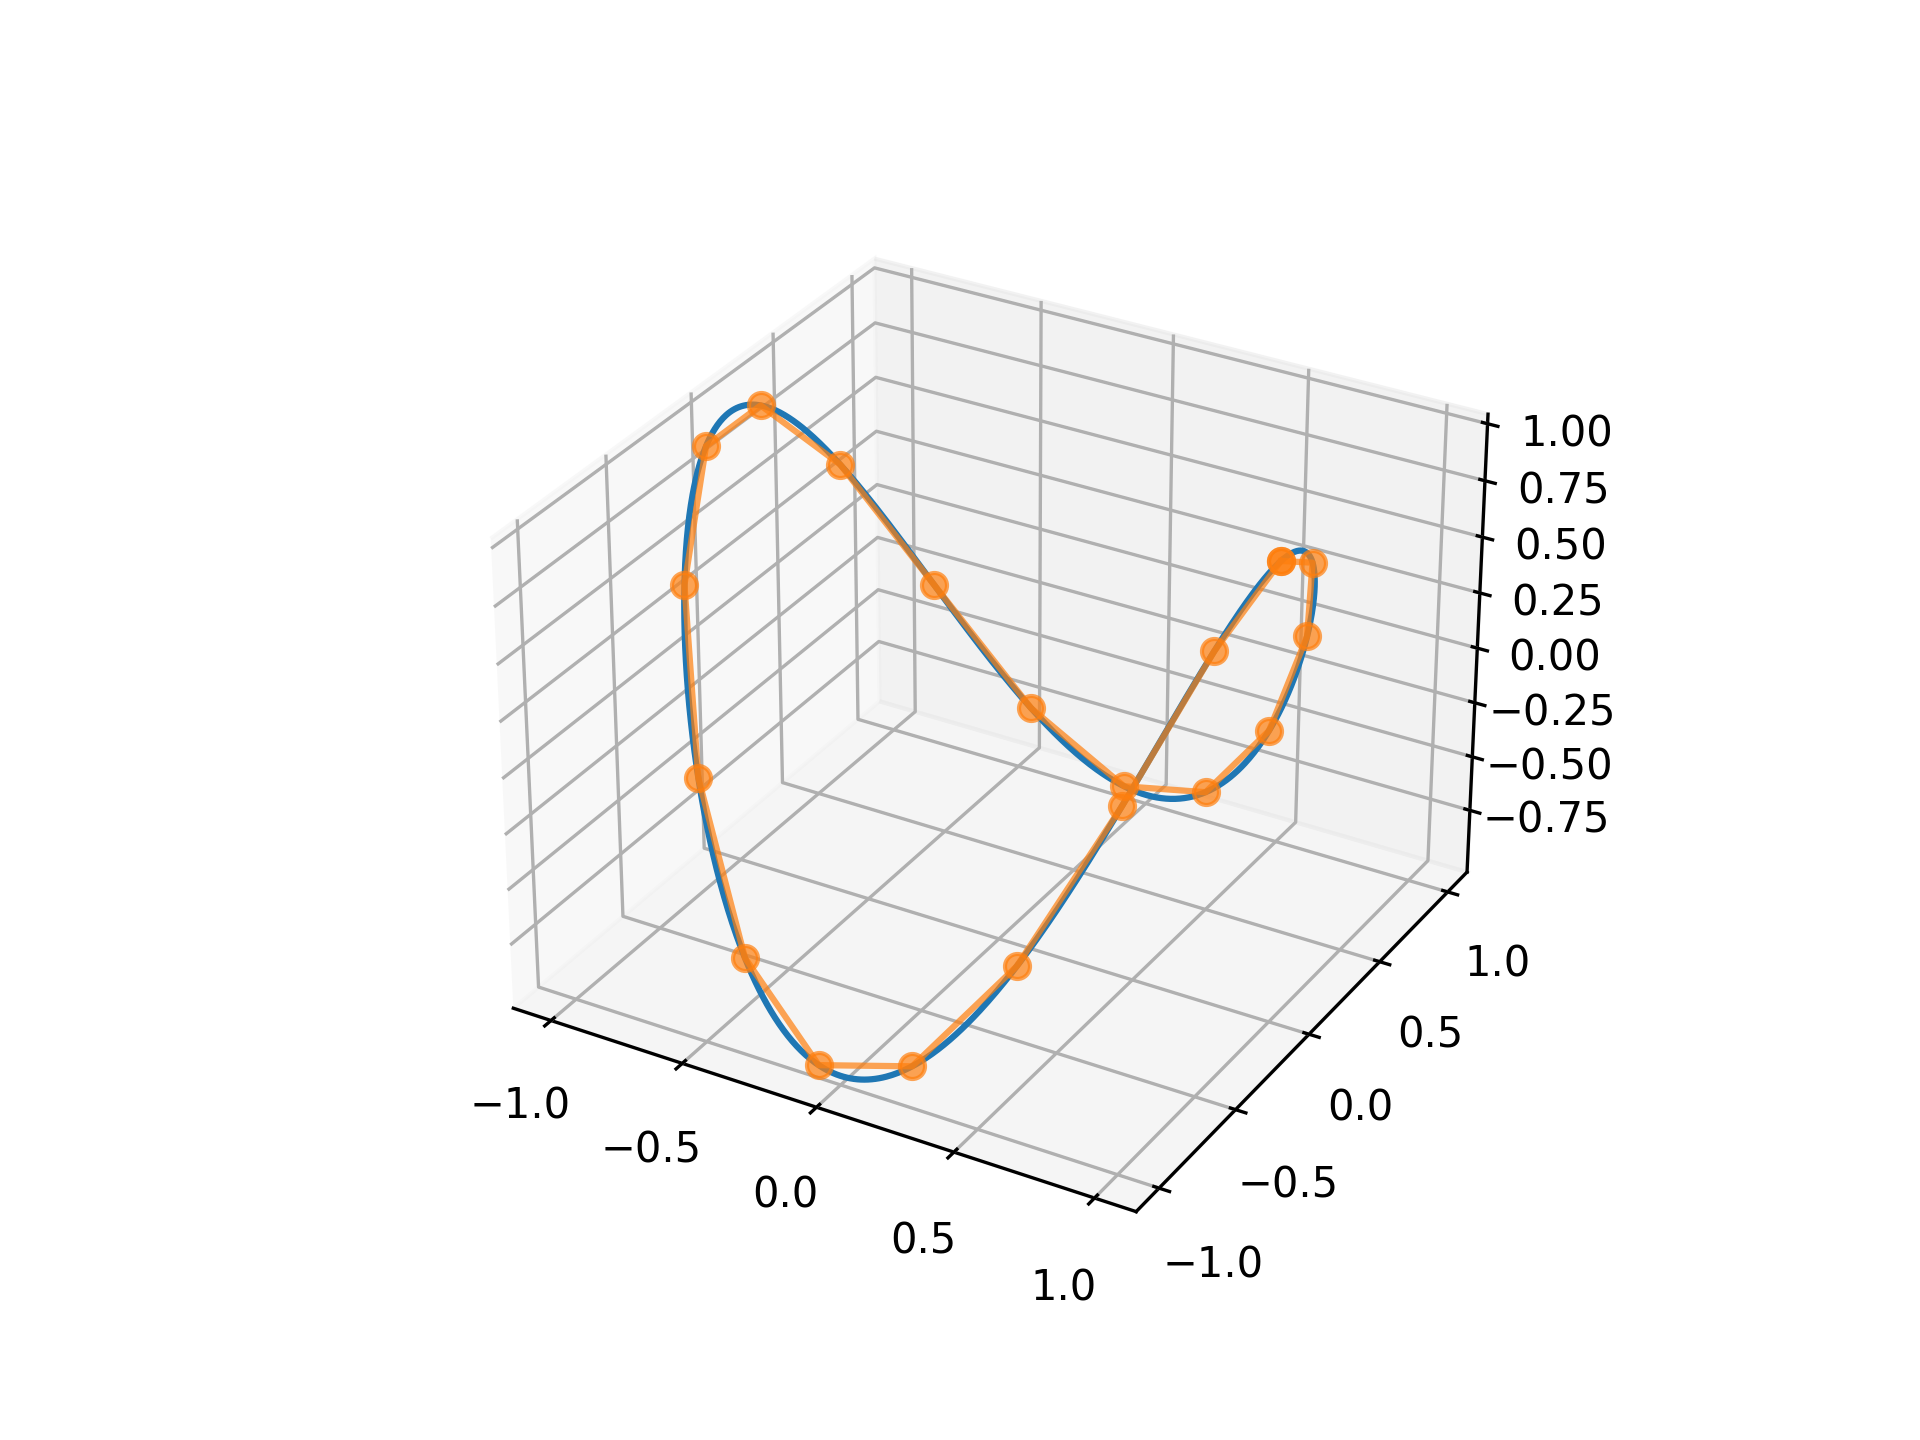
\includegraphics[width=0.8\textwidth]{sections/discretizationImgs/discretization}
    \caption{Discretisation of a simple closed curve by sampling the points along the curve.}
    \label{fig: Discretization of Curve}
\end{figure}

One way to resolve the issue is to ``ignore'' the adjacent edge contribution\cite{YSC2021} in the energy quadrature $E_{\beta}^{\alpha}$ as shown in Figure \ref{fig: Energy discretization by ignoring adjacent edges}.
The justification is that as we take a finer mesh ($N$ sufficiently large), the product of edge lengths ($\norm{e_i}\norm{e_j}$) should tend to zero sufficiently fast, resulting in approximation of the energy for the smooth curve, which did not have vertices resulting in local non-integrability in the first place.
\begin{figure}[tbp]
    \centering
    \begin{subfigure}[b]{0.75\textwidth}
        \centering
        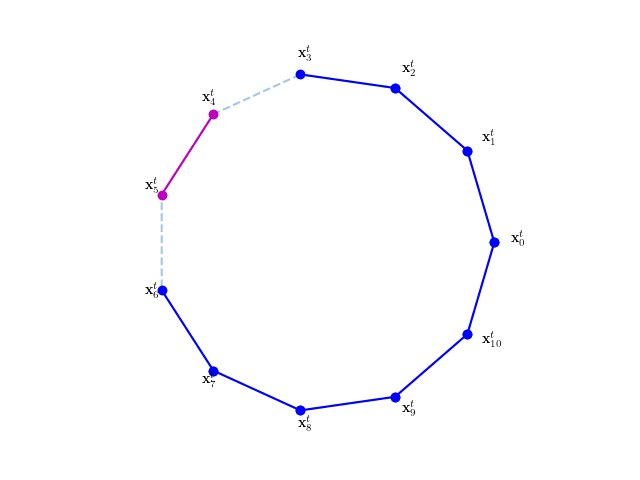
\includegraphics[width=\textwidth]{sections/unknottingCurveImgs/energyDiscretization1}
        \caption{For a chosen edge $e_i^k$, ignore the two adjacent edges $e_{i-1}^k$, $e_{i+1}^k$.
            In the limit as $N \rightarrow 0$, because the edge lengths tend to zero,
            the discrepancy between the quadrature and the analytical value of the energy is expected to tend to zero.
                }
        \label{fig: Energy discretization by ignoring adjacent edges}
    \end{subfigure}
    \par\bigskip
    \begin{subfigure}[b]{0.75\textwidth}
        \centering
        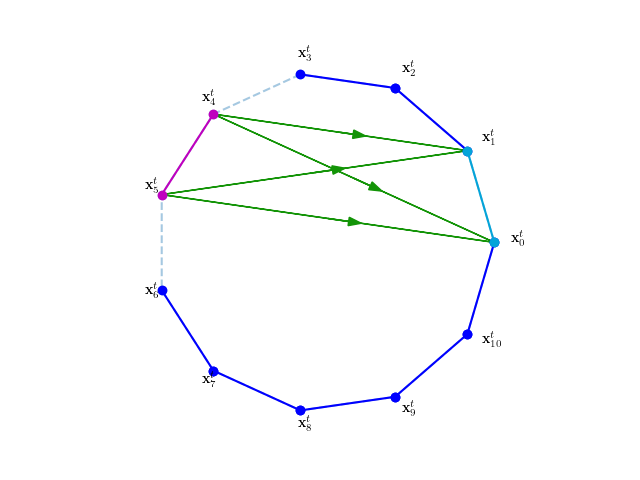
\includegraphics[width=\textwidth]{sections/unknottingCurveImgs/energyDiscretization2}
        %\caption{Tangent-point kernel is approximated by 4-point quadrature $K_\beta^\alpha (i, j)$ defined as (\ref{equ: Kernel 4-point}).}
        \caption{Tangent-point kernel is approximated by 4-point quadrature defined as (\ref{equ: Kernel 4-point}).}
        \label{fig: Tangent-point kernel approximation}
    \end{subfigure}
    \caption{Quadrature for approximation of tangent-point energy.}
\end{figure}

It still remains to sensibly approximate the kernel $k_{\beta}^{\alpha} (\gammabf_x, \gammabf_y) \approx K_{\beta}^{\alpha} (i, j)$.
One sensible approximation is to use the following 4-point quadrature\cite{YSC2021} (See Figure \ref{fig: Tangent-point kernel approximation}):
\begin{multline}
    K_{\beta}^{\alpha} (i, j) \coloneqq \frac{1}{4} \biggl( k_{\beta}^{\alpha} \left( \xbf_i^k, \xbf_j^k, \Tbf_i^k \right)
        + k_{\beta}^{\alpha} \left( \xbf_i^k, \xbf_{j+1}^k, \Tbf_i^k \right) \\
        + k_{\beta}^{\alpha} \left( \xbf_{i+1}^k, \xbf_j^k, \Tbf_i^k \right)
        + k_{\beta}^{\alpha} \left( \xbf_{i+1}^k, \xbf_{j+1}^k, \Tbf_i^k \right)
    \biggr)
    \label{equ: Kernel 4-point}
\end{multline}
where $\Tbf_{i}^k \coloneqq \frac{\xbf_{i+1}^k - \xbf_i^k}{\norm{\xbf_{i+1}^k - \xbf_i^k}}$ approximates the tangent vector to the curve at $\gammabf_x$.

Putting (\ref{equ: Energy Approximation Form}) and (\ref{equ: Kernel 4-point}) together,
one can write the \textbf{tangent-point energy quadrature} as:
\begin{equation}
    E_{\beta}^{\alpha} \coloneqq \sum_{\substack{i, j \in \left\{ 0, \cdots, N-1 \right\} \\ r \left( i-j,N \right) > 1}} K_{\beta}^{\alpha} (i,j) \norm{e_i^k} \, \norm{e_j^k}
    \label{equ: Tangent-Point Energy Quadrature}
\end{equation}
where $r\left( i-j,N \right)$ is the geodesic distance between $i$ and $j$ in modulo $N$,
characterising the avoidance of adjacent edges on simple closed polygonal curve.



\subsubsection{Finite Difference Scheme of Curve Untangling Process}
Based on (\ref{equ: Curve Untangling Process}), one writes the following finite difference scheme:
\begin{equation}
    \mathcal{D}_{t} \Gammabf^{k} = -\grad_{\mathcal{X}} E_{\beta}^{\alpha} (\Gammabf^k) - \grad_{\mathcal{X}} C \left( \Gammabf^k \right) \hspace{1cm} \text{for } k=0,1,\cdots
\end{equation}
where $\mathcal{D}_t$ is the finite difference operator over time step.
For the simplest scheme, one could take the forward difference operator as $\mathcal{D}_t \Gammabf^k(i) \coloneqq \frac{\Gammabf^{k+1}(i) - \Gammabf^{k}(i)}{\Delta T}$.

\subsection{$L^2$ Explicit Euler Scheme}

\end{document}
